\documentclass{article}

\usepackage{tikz}
\usepackage{amsmath}
\usepackage{amssymb}
\usepackage{bm}
\usetikzlibrary{bayesnet}

\newcommand\numberthis{\addtocounter{equation}{1}\tag{\theequation}}
\DeclareMathOperator*{\argmax}{arg\,max}

\title{IRL with Positive and Negative Labels}
\author{James MacGlashan}

\date{}

\begin{document}

\maketitle

\section{Problem Statement}
In this document we propose a variant of the inverse reinforcement learning problem. The learning problem is defined as being given a dataset of labeled trajectories and outputting a reward function, where each trajectory is a sequence of state-action pairs and each trajectory label is a positive ($+1$), or negative ($-1$) label that indicates whether the associated trajectory is a good example of some desired behavior, or a bad example of some desired behavior. The goal is to recover a reward function that motivates good behavior. In particular, we adopt the probabilistic maximum likelihood formulation, in which we seek a reward function that maximizes the likelihood of the data.

\section{Probability Model}
To find the reward function that maximizes the likelihood of the data, we first define probability model of the system that is represented in Figure~\ref{fig:gm}. The motivation for this model is that we consider the the final label ($L$) that a user gives a trajectory of size $N$ to be some random function of what they thought about each of the action selections ($A$) exhibited in the trajectory. However these step-wise evaluations ($X$) are unobserved in the data.
\begin{figure}
\centering
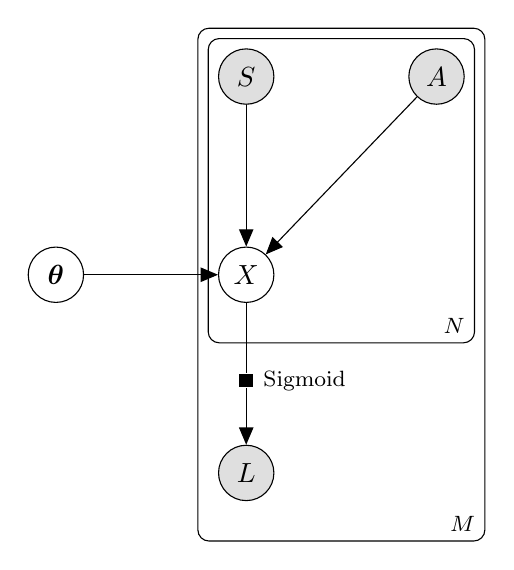
\begin{tikzpicture}[x=1.7cm,y=1.8cm]
   \node[latent]                   (R)      {$\bm{\theta}$} ; %
   \node[latent, right=of R]                   (X)      {$X$} ; %
   \node[obs, below=of X]                      (L)      {$L$} ; %
   \node[obs, above=of X]          (S)      {$S$} ; %
   \node[obs, right=of S]          (A)      {$A$} ; %
   
   \factor[above=of L]{L-f}{right:Sigmoid}{}{} ;

  \edge {S}{X} ;
  \edge {A}{X} ;
  \edge {R}{X} ;
  \factoredge {X}{L-f}{L} ;

   \plate {traj}{
   		(S) (A) (X)
   } {$N$} ;%

   \plate {data}{
   		(traj)(L-f)(L)
   } {$M$} ;

\end{tikzpicture}
\caption{Plate Diagram of our Probability Model}
\label{fig:gm}
\end{figure}

We model the probability that an action is evaluated as good or not as proportional to its selection probability according a softmax policy computed for the reward function with parameters $\bm{\theta}$. Specifically:
\begin{align}
\Pr(x_i = +1 | s, a, \theta) &= \pi(s, a | \bm{\theta}) \\
\Pr(x_i = -1 | s, a, \theta) &= 1 - \pi(s, a | \bm{\theta}),
\end{align}
where $\pi(s, a | \bm{\theta})$ is the softmax policy over Q-values computed for the reward function parameterized by $\bm{\theta}$:
\begin{equation}
\pi(s, a | \bm{\theta}) = \frac{e^{\beta Q(s,a | \bm{\theta})}}{\sum_{a'}e^{\beta Q(s,a' | \bm{\theta})}},
\end{equation}
$\beta$ is a selectable parameter, and $Q(s,a|\bm{\theta})$ is the Q-value computed for the reward function parameterized by $\bm{\theta}$.


For the probability distribution of $L$, given the sequence of $N$ step-wise labels, we would like a distribution that has the property that as more step-wise labels are positive, the probability of a positive trajectory label increases (and vice versa). Although there are many possible distributions that satisfy this property, for concreteness, we choose the sigmoid function. That is,
\begin{align}
\Pr(L = +1 | X_1, ..., X_n) &= \frac{1}{1 + e^{-\phi \sum_i^N X_i}} \\
\Pr(L = -1 | X_1, ... ,X_n) &= 1 - \Pr(L = +1 | X_1, ..., X_n),
\end{align}
where $\phi$ is a selectable parameter that tunes how quickly of a majority of step-wise labels increases/decreases the probability of trajectory assignment. For example, when $\phi = 0$, trajectory labels are assigned uniformly randomly independently of step-wise labels. As $\phi \rightarrow \infty$, the sigmoid converges to a step function in which a trajectory containing even one more positive step-wise label than negative step-wise labels will deterministically cause a positive trajectory label (and vice versa).

\section{Finding the Parameters that Maximum the Likelihood}
Recall that our goal is to find the maximum likelihood reward function parameters given a dataset with $M$ trajectories (sequences of $S,A$ pairs) and trajectory labels ($L$), but {\em not} step-wise labels ($X$). Under our model, the likelihood of such a dataset $D$ of size $M$ for a given set of reward function parameters $\theta$ is
\begin{align*}
\mathcal{L}(D | \bm{\theta}) &= \prod_i^M \Pr(l_i, s_{i,1}, a_{i,1} ..., s_{i,N}, a_{i,N}| \bm{\theta}) \\
&= \prod_i^M \sum_{\mathbf{x} \in \{-1, 1\}^N} \Pr(l_i, s_{i,1}, a_{i,1}, x_1, ..., s_{i,N}, a_{i,N}, x_N | \bm{\theta}) \\
&= \prod_i^M \sum_{\mathbf{x} \in \{-1, 1\}^N} \Pr(l_i | x_1, ..., x_n) \Pr(x_1, ..., x_N | s_{i,1}, a_{i,1}, ..., s_{i,N}, a_{i,N}, \bm{\theta}) \\
&= \prod_i^M \sum_{\mathbf{x} \in \{-1, 1\}^N} \Pr(l_i | x_1, ..., x_n) \prod_j^N \Pr(x_j | s_{i,j}, a_{i,j}, \bm{\theta}) \numberthis \label{eq:likelihood}
\end{align*}

We will estimate the maximum likelihood parameters by using gradient ascent to (locally) maximize the log likelihood function, where the log likelihood is:
\begin{align*}
\log \mathcal{L}(D | \bm{\theta}) &= \sum_i^M \log \sum_{\mathbf{x} \in \{-1, 1\}^N} \Pr(l_i | x_1, ..., x_n) \prod_j^N \Pr(x_j | s_{i,j}, a_{i,j}, \bm{\theta}) \\
&= \sum_i^M q_i + \log \left[ \sum_{\mathbf{x} \in \{-1, 1\}^N} \exp \left(-q_i + \log \left( \Pr(l_i | x_1, ..., x_n) \prod_j^N \Pr(x_j | s_{i,j}, a_{i,j}, \bm{\theta}) \right) \right) \right] \\
&= \sum_i^M q_i + \log \left[ \sum_{\mathbf{x} \in \{-1, 1\}^N} \exp \left(-q_i + \log \left( \Pr(l_i | x_1, ..., x_n) \right) + \sum_j^N \log \left( \Pr(x_j | s_{i,j}, a_{i,j}, \bm{\theta}) \right) \right) \right],
\end{align*}
where 
\begin{align*}
q_i = \max_{\mathbf{x} \in \{-1, 1\}^N} \log \left( \Pr(l_i | x_1, ..., x_n) \right) + \sum_j^N \log \left( \Pr(x_j | s_{i,j}, a_{i,j}, \bm{\theta}) \right).
\end{align*}

To simplify the expression of this function, and make the gradient more clear, we will break the log likelihood function up into different sub-functions, which are all implicitly defined with respect to a $\bm{\theta}$. Let
\begin{align}
P_{xij} &= \begin{cases}
\pi(s_{i,j}, a_{i,j} | \bm{\theta}) & \mbox{if } x_{i,j} = 1 \\
1 - \pi(s_{i,j}, a_{i,j} | \bm{\theta}) & \mbox{if } x_{i,j} = -1
\end{cases} \\
net_{x} &= \phi \sum_j^N x_{j} \\
S(x) &= \frac{1}{1 + e^{-x}} \\
P_{lix} &= \begin{cases}
S(net_{xi}) & \mbox{if } l = 1 \\
1 - S(net_{xi}) & \mbox{if } l = -1
\end{cases} \\
g_{xi} &= \log P_{lix} + \sum_j^N \log P_{xij} \\
m_i &= \argmax_{\mathbf{x} \in \{-1, 1\}^N} g_{xi} \\
f_{xi} &= g_{xi} - g_{m_ii}.
\end{align}
Then, using these terms, we can rewrite the log likelihood as
\begin{equation}
\log \mathcal{L}(D | \bm{\theta}) = g_{m_ii} + \log \sum_{\mathbf{x} \in \{-1, 1\}^N} e^{f_{xi}}.
\end{equation}
The partial derivative for any single parameter $\theta$ of $\bm{\theta}$ of the log likelihood under this expression is
\begin{equation}
\frac{\partial}{\partial \theta} \log \mathcal{L}(D | \bm{\theta}) = \frac{\partial}{\partial \theta} g_{m_ii} + \frac{\sum\limits_{\mathbf{x} \in \{-1, 1\}^N} \left( e^{f_{xi}} \right) \frac{\partial}{\partial \theta} f_{xi}}{\sum\limits_{\mathbf{x} \in \{-1, 1\}^N} e^{f_{xi}}}.
\end{equation}
We will compute the partial partial derivatives for each of these terms by examining the partial derivatives for each of our sub functions, bottom up.
\begin{align}
\frac{\partial}{\partial \theta} net_{x} &= 0 \\
\frac{\partial}{\partial \theta} S(net_x) &= S(net_x)(1 - S(net_x))\frac{\partial}{\partial \theta} net_x \nonumber \\
&= S(net_x)(1 - S(net_x)) 0 \nonumber \\
&= 0 \\
\frac{\partial}{\partial \theta} P_{lix} &= \begin{cases}
\frac{\partial}{\partial \theta} S(net_x) & \mbox{if } l = 1 \\
-\frac{\partial}{\partial \theta} S(net_x) & \mbox{if } l = -1
\end{cases} \nonumber \\
&= 0 \\
\frac{\partial}{\partial \theta} P_{xij} &= \begin{cases}
\frac{\partial}{\partial \theta} \pi(s_{i,j}, a_{i,j} | \bm{\theta}) & \mbox{if } x_{i,j} = 1 \\
-\frac{\partial}{\partial \theta} \pi(s_{i,j}, a_{i,j} | \bm{\theta}) & \mbox{if } x_{i,j} = -1
\end{cases} \\
\frac{\partial}{\partial \theta} g_{xi} &= \frac{\frac{\partial}{\partial \theta} P_{lix}}{P_{lix}} + \sum_j^N \frac{\frac{\partial}{\partial \theta} P_{xij}}{P_{xij}} \nonumber \\
&= \sum_j^N \frac{\frac{\partial}{\partial \theta} P_{xij}}{P_{xij}} \\
\frac{\partial}{\partial \theta} f_{xi} & = \frac{\partial}{\partial \theta} g_{xi} - \frac{\partial}{\partial \theta} g_{m_ii}.
\end{align}

It is interesting to note that the partial derivative of the probability distribution for the $L$ function goes to zero. This result is due to the fact that once some set of $X$ values have been selected, the likelihood does not depend on $\bm{\theta}$, and in the likelihood function, $X$ values are bound during the marginalization process in which we sum over them. However, it should be noted that just because the partial derivative for $L$ is zero, that does not mean that its probability distribution plays no role in the full partial derivative of the log likelihood. You will find the probability of $L$ given the $X$s non-differentiated value appearing in the exponentiation of our $f_{xi}$ terms.

Finally, in this document, I did not provide the partial derivative of the policy, which in turn depends on the partial derivative of the Q-function. However, these terms have been explained in existing IRL work that we can reuse.


\section{Importance Sampling}

Recall likelihood.
\begin{equation}
\mathcal{L}(D \mid \theta) = \prod_i^M \sum_{\mathbf{x} \in \{-1, 1\}^N} \Pr(l_i | x_1, ..., x_n) \prod_j^N \Pr(x_j | s_{i,j}, a_{i,j}, \bm{\theta})
\end{equation}
Is also equal to...
\begin{equation}
\mathcal{L}(D \mid \theta) = \prod_i^M \sum_{\mathbf{x} \in \{-1, 1\}^N} \Pr(l_i | x_1, ..., x_n) \prod_j^N \Pr(x_j | s_{i,j}, a_{i,j}, \bm{\theta}) \frac{\zeta(\bm{x})}{\zeta(\bm{x})}
\end{equation}
Now we Monte-Carlo sample according to $q$
\begin{equation}
\hat{\mathcal{L}}(D \mid \theta) = \prod_i^M \frac{1}{C} \sum_k^C \frac{\Pr(l_i | x_1, ..., x_n) \prod_j^N \Pr(x_j | s_{i,j}, a_{i,j}, \bm{\theta})}{\zeta(\bm{x})}
\end{equation}
Now we do log likelihood
\begin{align*}
\log \hat{\mathcal{L}}(D | \bm{\theta}) &= \sum_i^M \log \frac{1}{C} \sum_k^C \frac{\Pr(l_i | x_1, ..., x_n) \prod_j^N \Pr(x_j | s_{i,j}, a_{i,j}, \bm{\theta})}{\zeta(\bm{x})} \\
&= \sum_i^M  \log \frac{1}{C} + q_i + \log \left[ \sum_k^C \exp \left(-q_i + \log \left( \frac{\Pr(l_i | x_1, ..., x_n) \prod_j^N \Pr(x_j | s_{i,j}, a_{i,j}, \bm{\theta})}{\zeta(\bm{x})} \right) \right) \right] \\
&= \sum_i^M \log \frac{1}{C} + q_i + \log \left[ \sum_k^C \exp \left(-q_i -\log\zeta(\bm{x}) + \log \left( \Pr(l_i | x_1, ..., x_n) \right) + \sum_j^N \log \left( \Pr(x_j | s_{i,j}, a_{i,j}, \bm{\theta}) \right) \right) \right],
\end{align*}
where,
\begin{align*}
q_i = \max_{\mathrm{samples}} -\log\zeta(\bm{x}) + \log \left( \Pr(l_i | x_1, ..., x_n) \right) + \sum_j^N \log \left( \Pr(x_j | s_{i,j}, a_{i,j}, \bm{\theta}) \right).
\end{align*}




\end{document}